%!TEX root = ../../main.tex
For the handwriting to be effective we had to bring the data into a clean state. To this end we used a pipeline which is described below in figure \ref{fig:pipeline}. 

\begin{figure}[ht]
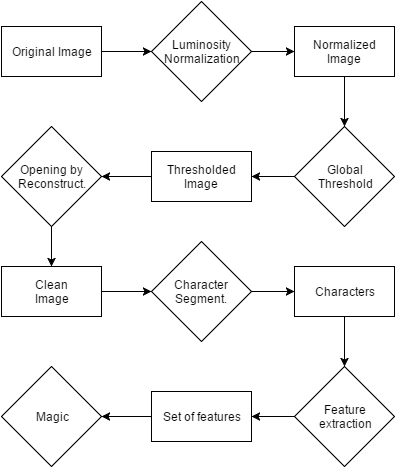
\includegraphics[width=8cm]{shared/img/pipeline.png}
\caption{Overview of our pipeline.}
\label{fig:pipeline}
\end{figure}

\subsubsection{Luminosity}

The luminosity normalization is essential for the thresholding to work since in some parts of dataset the ink has worn off the pages. Figure \Cref{fig:methods:preprocessing:lumNormalization} gives an example why luminosity normalization was necessary. In the above mentioned figure, we applied the same threshold filter with and without luminosity normalization and the results speak for themselves. By normalizing the luminosity we eliminate the need to adjust threshold values in later steps.

\begin{figure}
	\centering
	\subfloat[]{
		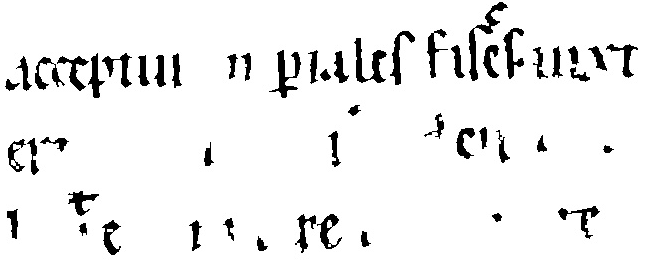
\includegraphics[width=\columnwidth]{shared/img/before_lum.png}%
		\label{fig:methods:preprocessing:lumNormalization:before}%
	}
	\hfil
	\subfloat[]{
		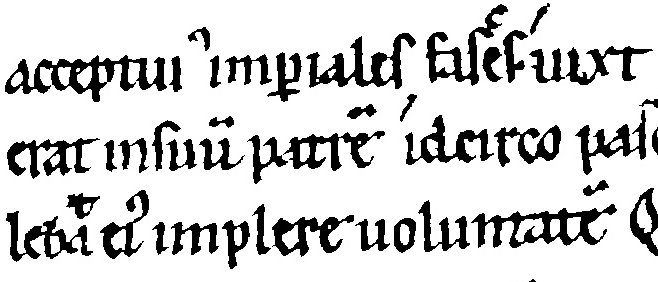
\includegraphics[width=\columnwidth]{shared/img/after_lum.png}%
		\label{fig:methods:preprocessing:lumNormalization:after}%
	}
	\caption{An image of text \protect\subref{fig:methods:preprocessing:lumNormalization:before} before and \protect\subref{fig:methods:preprocessing:lumNormalization:after} after luminization normalization.}
	\label{fig:methods:preprocessing:lumNormalization}
\end{figure}

\subsubsection{Binarization and Morphological operations}

The next step is to binarize the image. For the binarization we tested both the Otsu approach and global threshold and we settled with the former as it gave better results which resulted to its use. Finally we use morphological operations on the image to remove whatever noise might have left behind. This morphological operation allowed us to keep large components in the image such as are the letters while completely removing smaller comportments such as some noise dots. In mathematical morphology, the closing of a set (binary image) $A$ by a structuring element $B$ is the erosion of the dilation of that set. In mathematical terms we can formulate the closing as:
\begin{equation}
A \bullet B = (A \oplus B) \ominus B.
\end{equation}
During the processes however we ended up missing some punctuation points which however did not provide crucial to our recognizer. In figure \ref{fig:methods:preprocessing} we can see the final result with Otsu and global thresholding.

\begin{figure}
	\centering
	\subfloat[]{
		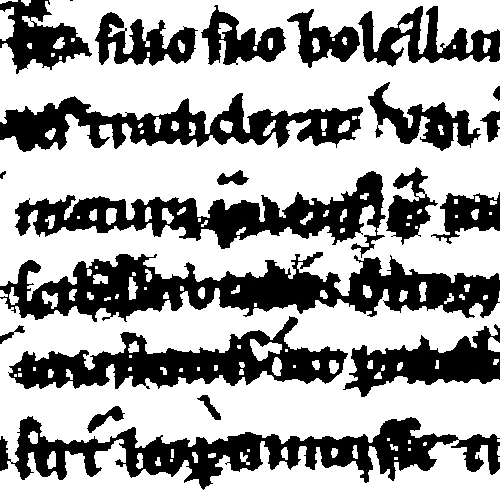
\includegraphics[width=\columnwidth]{shared/img/reco_thres.png}%
		\label{fig:methods:preprocessing:thres}%
	}
	\hfil
	\subfloat[]{
		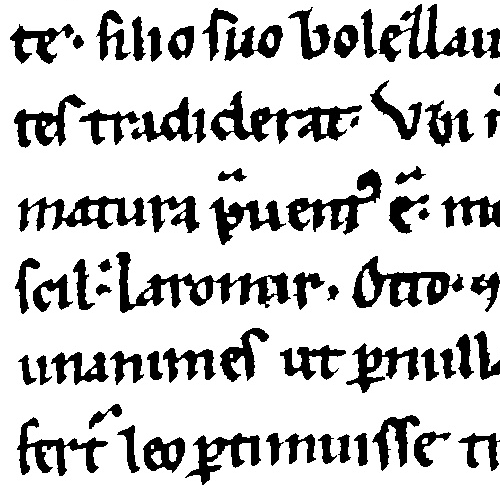
\includegraphics[width=\columnwidth]{shared/img/reco_otsu.png}%
		\label{fig:methods:preprocessing:otsu}%
	}
	\caption{Result with global threshold (threshold value 170) and opening by reconstruction \protect\subref{fig:methods:preprocessing:thres}. Result with Otsu and opening by reconstruction \protect\subref{fig:methods:preprocessing:otsu}.}
	\label{fig:methods:preprocessing}
\end{figure}

At this point it is worth noting that the size of the mask we used for the erosion was a 7 by 7 whereas the mask for the dilation was only 3 by 3. This was done on purpose in order to achieve higher accuracy in the final results.